\documentclass[11pt]{article}
\usepackage[T1]{fontenc}
\usepackage[margin=0.82in]{geometry}
\usepackage{amsmath,amssymb}
\usepackage{booktabs,tabularx}
\usepackage{graphicx}
\usepackage[hidelinks]{hyperref}
\usepackage{microtype}

\newcommand{\R}{\mathbb R}
\newcommand{\Sph}{\mathbb S}

\title{The low-dimensional second-order Hydrogen uncertainty conjecture}
\author{Literature-already-answered note for arXiv:2012.12667}
\date{12 August 2026}

\begin{document}
\maketitle

\paragraph{Status.}
\textbf{The conjecture is false in dimensions $2$ and $3$.}
Chen--Tang prove this in arXiv:2508.15221, Theorem~1.1; their
first-spherical-harmonic test gives a strict counterexample.  The
remaining dimension $4$ was subsequently answered affirmatively by
Huang--Ye, arXiv:2510.00453, Theorem~1.2.  Thus the later literature now
settles the entire range $2\le N\le4$.

\section*{The source conjecture}
For $u\in W^{2,2}(\R^N)$ set
\[
 Q_N[u]:=
 \frac{\displaystyle\int_{\R^N}|\Delta u|^2,dx
                   \displaystyle\int_{\R^N}|\nabla u|^2,dx}
      {\left(\displaystyle\int_{\R^N}
             \frac{|\nabla u|^2}{|x|},dx\right)^2}.
\]
Theorem~2.3 of arXiv:2012.12667 proves
$Q_N[u]\ge (N+1)^2/4$ for $N\ge5$, sharply.  Remark~2.4 on source PDF
page~5 conjectures that the same inequality holds for $2\le N\le4$.

\begin{center}

\includegraphics[width=0.88\textwidth]{evidence/source_conjecture_crop.png}

{\footnotesize Source evidence: arXiv:2012.12667, PDF page 5 (unaltered crop).}
\end{center}

\clearpage
\section*{The exact later counterexample}
Chen--Tang's Theorem~1.1 (supporting PDF page~5) proves that for
$N\in\{2,3\}$ the sharp constant $C(N)=\inf_{u\ne0}Q_N[u]$ satisfies
\[
 \frac{(N-1)^4(N+3)^2}{4(N^2-2N+5)^2}
 \le C(N)\le
 \frac{N(N+4)(N^2-1)^2}{4(N^2-N+4)^2}
 <\frac{(N+1)^2}{4}.
\]
The final strict inequality is a direct negative answer to the source
conjecture.

\begin{center}
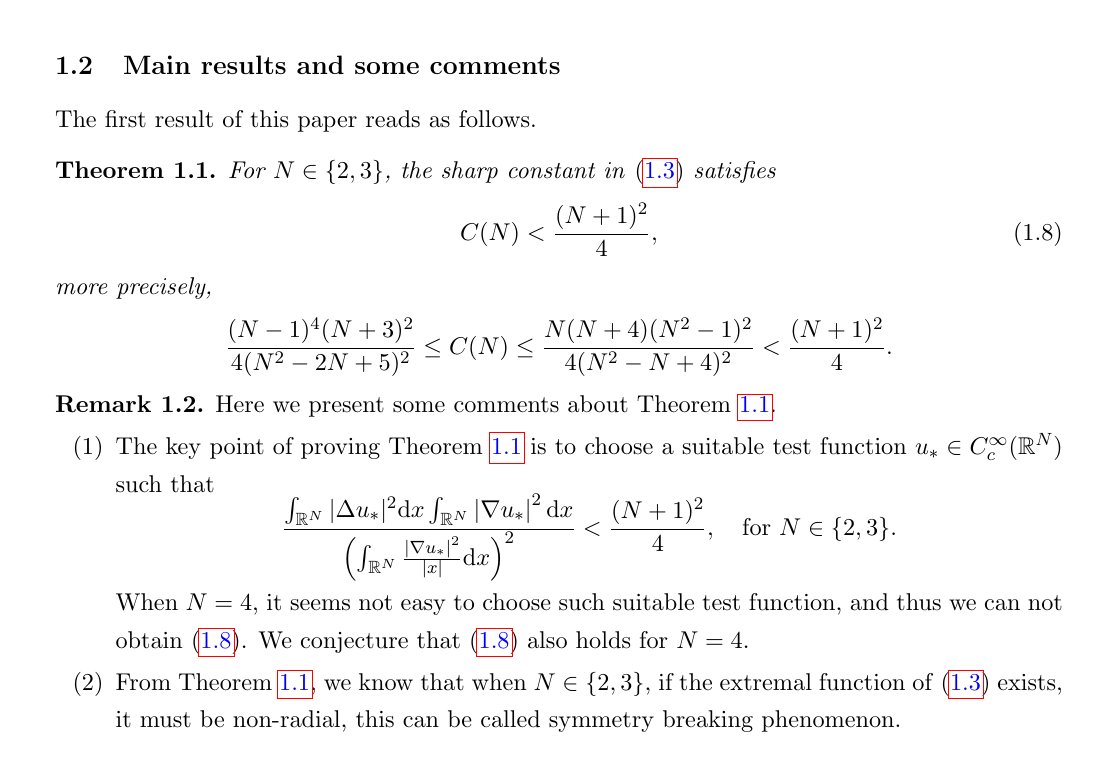
\includegraphics[width=0.88\textwidth]{evidence/support2508_theorem_crop.png}

{\footnotesize Later-answer evidence: arXiv:2508.15221, Theorem 1.1 on PDF
page 5 (unaltered crop).}
\end{center}

\section*{Transparent verification of the test}
Take a degree-one spherical harmonic $\phi$ and
\[
 u_*(r\sigma)=r e^{-r}\phi(\sigma).
\]
Up to a harmless angular normalization this is $u_*(x)=x_1e^{-|x|}$.
It belongs to $W^{2,2}(\R^N)$ for $N\ge2$; standard cutoff and smoothing
also place it in the closure of $C_c^\infty$ under the relevant Sobolev
norm.  Writing $K=\int_{\Sph^{N-1}}|\phi|^2,d\sigma$, spherical-harmonic
identities give
\begin{align*}
 \int|\Delta u_*|^2
 &=K\left(\frac{\Gamma(N+2)}{2^{N+2}}
       +(N+1)\frac{\Gamma(N)}{2^N}\right),\\
 \int|\nabla u_*|^2
 &=K\frac{\Gamma(N+2)}{2^{N+2}},\\
 \int\frac{|\nabla u_*|^2}{|x|}
 &=K\left(\frac{\Gamma(N+1)}{2^{N+1}}
       +\frac{\Gamma(N-1)}{2^{N-1}}\right).
\end{align*}
The factor $K$ cancels, and $\Gamma(t+1)=t\Gamma(t)$ yields
\[
 Q_N[u_*]=
 \frac{N(N+4)(N^2-1)^2}{4(N^2-N+4)^2}.
\]
Consequently
\[
 Q_2[u_*]=\frac34<\frac94,
 \qquad
 Q_3[u_*]=\frac{84}{25}<4.
\]
Either value alone disproves the three-dimension-range conjecture; together
they display the symmetry breaking in both low dimensions.

\section*{Proof intuition}
The radial extremizer $(1+\beta r)e^{-\beta r}$ realizes the conjectured
constant, so a counterexample must be nonradial.  Spherical-harmonic
decomposition separates the three quadratic forms defining $Q_N$.  In the
first nonradial sector, $u=r v(r)\phi_1(\sigma)$, choosing $v=e^{-r}$ turns
every radial integral into a Gamma integral.  In $N=2,3$ the angular-energy
contribution enlarges the weighted denominator enough to push the quotient
strictly below the radial value.  This is precisely the symmetry-breaking
mechanism isolated by Chen--Tang.

\begin{center}
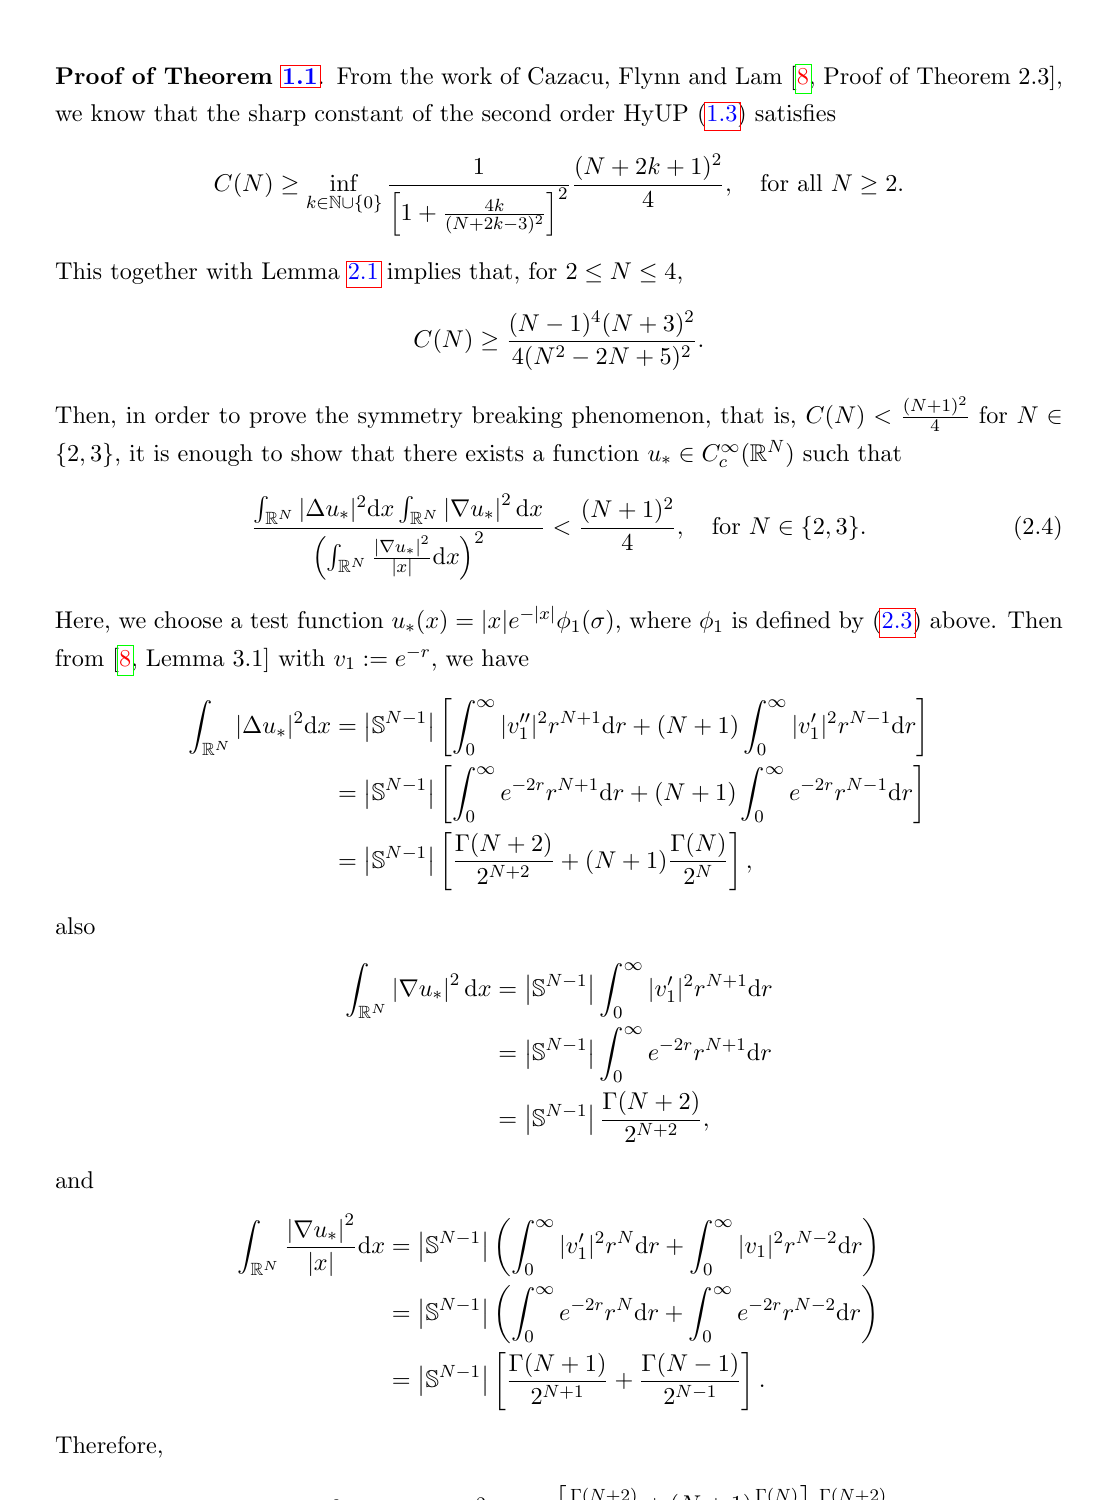
\includegraphics[width=0.55\textwidth]{evidence/support2508_test_crop.png}

{\footnotesize Chen--Tang's explicit test and Gamma-integral computation,
arXiv:2508.15221, PDF page 9 (unaltered crop).}
\end{center}

\section*{The remaining dimension}
The above test gives $Q_4[u_*]=225/32>25/4$, so it does not decide $N=4$.
Huang--Ye subsequently proved the positive result
\[
 Q_N[u]\ge\frac{(N+1)^2}{4}\qquad(N\ge4),
\]
with equality exactly at $\alpha(1+\beta r)e^{-\beta r}$.  Their
Theorem~1.2 therefore closes the last case left by Chen--Tang.

\begin{center}
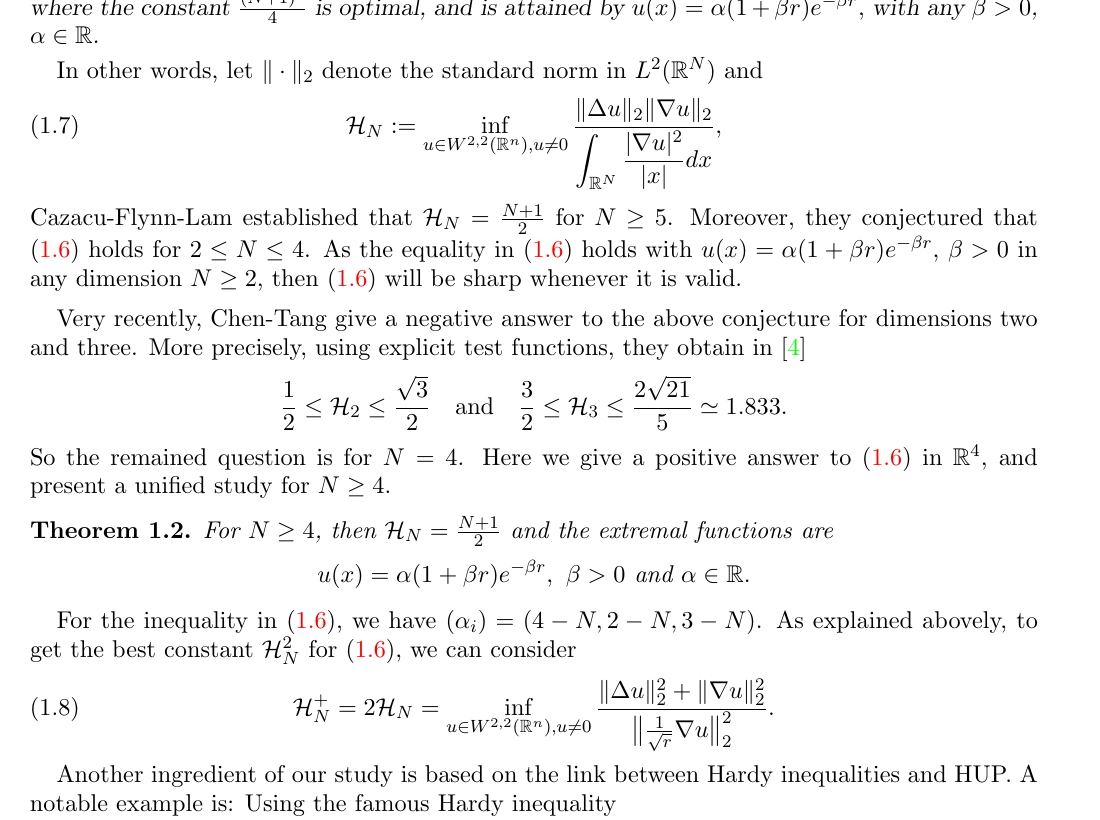
\includegraphics[width=0.74\textwidth]{evidence/support2510_n4_crop.png}

{\footnotesize Dimension-four closure: arXiv:2510.00453, Theorem 1.2 on PDF
page 3 (unaltered crop).}
\end{center}

\paragraph{Human review.}
Check Remark~2.4 on source PDF page~5, Chen--Tang Theorem~1.1 on supporting
PDF page~5 and its test computation on pages~9--10, and Huang--Ye
Theorem~1.2 on its PDF page~3.

\begin{thebibliography}{9}
\raggedright
\bibitem{source}
C. Cazacu, J. Flynn, and N. Lam,
\emph{Sharp second order uncertainty principles}, arXiv:2012.12667.

\bibitem{negative}
X.-P. Chen and C.-L. Tang,
\emph{On the extremal functions of second order uncertainty principles:
symmetry and symmetry breaking}, arXiv:2508.15221.

\bibitem{n4}
X. Huang and D. Ye,
\emph{On Sharp Heisenberg Uncertainty Principle and the stability},
arXiv:2510.00453.
\end{thebibliography}

\end{document}
